% !TEX root = main.tex

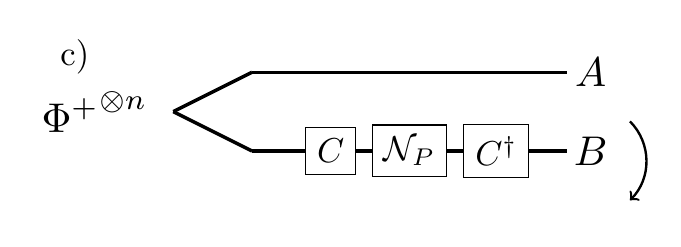
\begin{tikzpicture}
\node[scale=1.25] at (-1.25,0.7){c)};
\node[scale=1.5] at (-1,0){$\ket{\Phi^+}^{\otimes n}$};
\node[scale=1.5] at (5.3,1/2){$A$};
\node[scale=1.5] at (5.3,-1/2){$B$};
\draw[line width=1.25] (0,0) -- (1,1/2);
\draw[line width=1.25] (5,1/2) -- (1,1/2);
\draw[line width=1.25] (0,0) -- (1,-1/2);
\draw[line width=1.25] (5,-1/2) -- (1,-1/2);
\node[draw, scale=1.25, fill=white] at (3,-1/2){$\mathcal{N}_P$};
\node[draw, scale=1.25, fill=white] at (2,-1/2){$C$};
\node[draw, scale=1.25, fill=white] at (4.1,-1/2){$C^{\dagger}$};
\node[anchor=east] at (5.8, 0) (node1){};
\node[anchor=east] at (5.8, -1.25) (node2){};
\draw[->, line width=0.3mm] (node1) to [out = -45, in = 45, looseness = 1] (node2);
\end{tikzpicture}